

\chapter{Creación del Proyecto}


Los Tribunales Ambientales son órganos jurisdiccionales especiales, sujetos a la 
superintendencia directiva, correccional y económica de la Corte Suprema, cuya función 
es resolver las controversias medioambientales de su competencia y ocuparse de los 
demás asuntos que la ley somete a su conocimiento \cite{Ley20600}. Estos tribunales generan una cantidad 
de jurisprudencia que puede ser encontrada en su portal de consulta llamado buscador ambiental \cite{BuscadorAmbiental}. 

El proyecto consiste en la generación de un chatbot en donde se pueda preguntar sobre 
la jurisprudencia de estos tribunales, aunque por razones de capacidad el chatbot se 
vea acotado solamente a las reclamaciones recibidas por el tribunal.

Por lo que, este proyecto consiste en un proceso de extracción de datos 
desde el buscador ambiental, transformación de estos datos para su utilización, generación 
de vectores de estos datos para que puedan interaccionar con la aplicación, carga de estos 
en una base de datos, para que después la aplicación pueda interactuar con ellos y mandando 
esa información a el LLM, siendo en este caso gpt-4 perteneciente a OpenAI.

% Inclusión de Figuras
\begin{figure}[ht!]
    \centering
    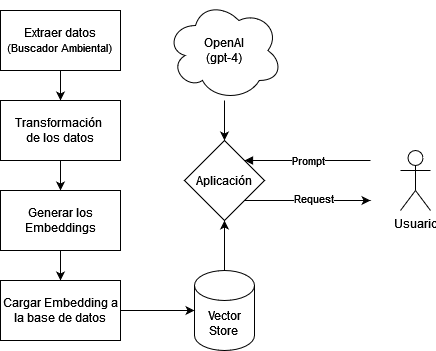
\includegraphics[width=.5\textwidth]{figures/huemul1.png}
    \caption[Estructura basica de la aplicación]{Estructura basica de la aplicación\\
    {\scriptsize (Fuente: Elaboración propia)}}
    \label{fig:logoind}
\end{figure}
    

A partir de esta estructura mientras se avance en el desarrollo, se explicará parte por parte el proceso y con ello los riesgos de cada uno de ellos.



\section{ETL}


Para realizar el proyecto fue necesario realizar un proceso de ETL. El término ETL se refiere a las técnicas de "Extracción, 
Transformación y Carga" (Extract, Transform, Load), que constituyen un proceso clave para los datos necesarios para el proyecto. 
Este proceso implica la extracción de datos de fuentes heterogéneas, su transformación para ajustarse a las necesidades del 
negocio y su posterior carga en un destino que, por lo general, es un almacén de datos diseñado para el análisis y la generación 
de informes\cite{ETL1}.

% Inclusión de Figuras
\begin{figure}[ht!]
    \centering
    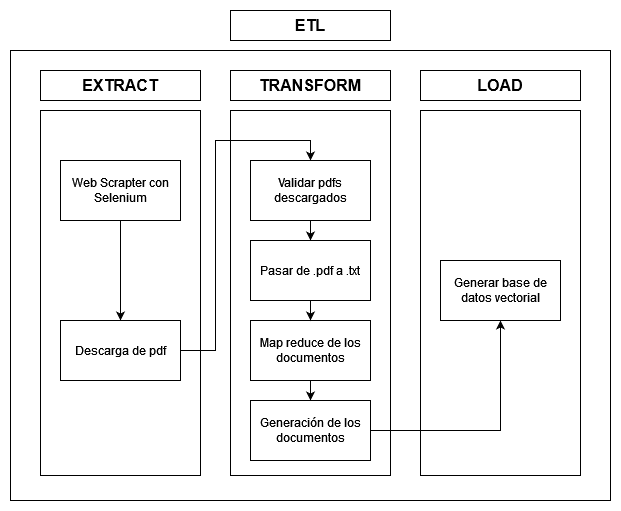
\includegraphics[width=.5\textwidth]{figures/huemulETL.png}
    \caption[Estructura del proceso de ETL para el Buscador Ambiental]{Estructura del proceso de ETL para el Buscador Ambiental\\
    {\scriptsize (Fuente: Elaboración propia)}}
    \label{fig:etl1}
\end{figure}
    

La fase de extracción implica la recolección de datos de múltiples fuentes, que pueden variar desde bases de datos 
estructuradas hasta información no estructurada en la web. La transformación se refiere al proceso de limpieza, conversión, 
y consolidación de estos datos en un formato adecuado para el análisis. Finalmente, la carga es el proceso de transferir 
los datos transformados al sistema de destino, donde se pueden almacenar y utilizar para la toma de decisiones estratégicas 
\cite{ETL1}.

\subsection{Extract}

%\autoref{fig:logoind}

La información requerida para el desarrollo del Chatbot se obtuvo del "Buscador ambiental" del Tribunal de Protección Ambiental 
de Chile a través de su sitio web\cite{BuscadorAmbiental}. Este portal aloja todos los documentos públicos disponibles para su consulta en cualquiera 
de los tres tribunales ambientales. Para acceder a la base de datos necesaria, se llevó a cabo la creación de 
un bot capaz de recopilar las entradas de este buscador de manera análoga a un usuario convencional.

\begin{figure}[ht!]
    \centering
    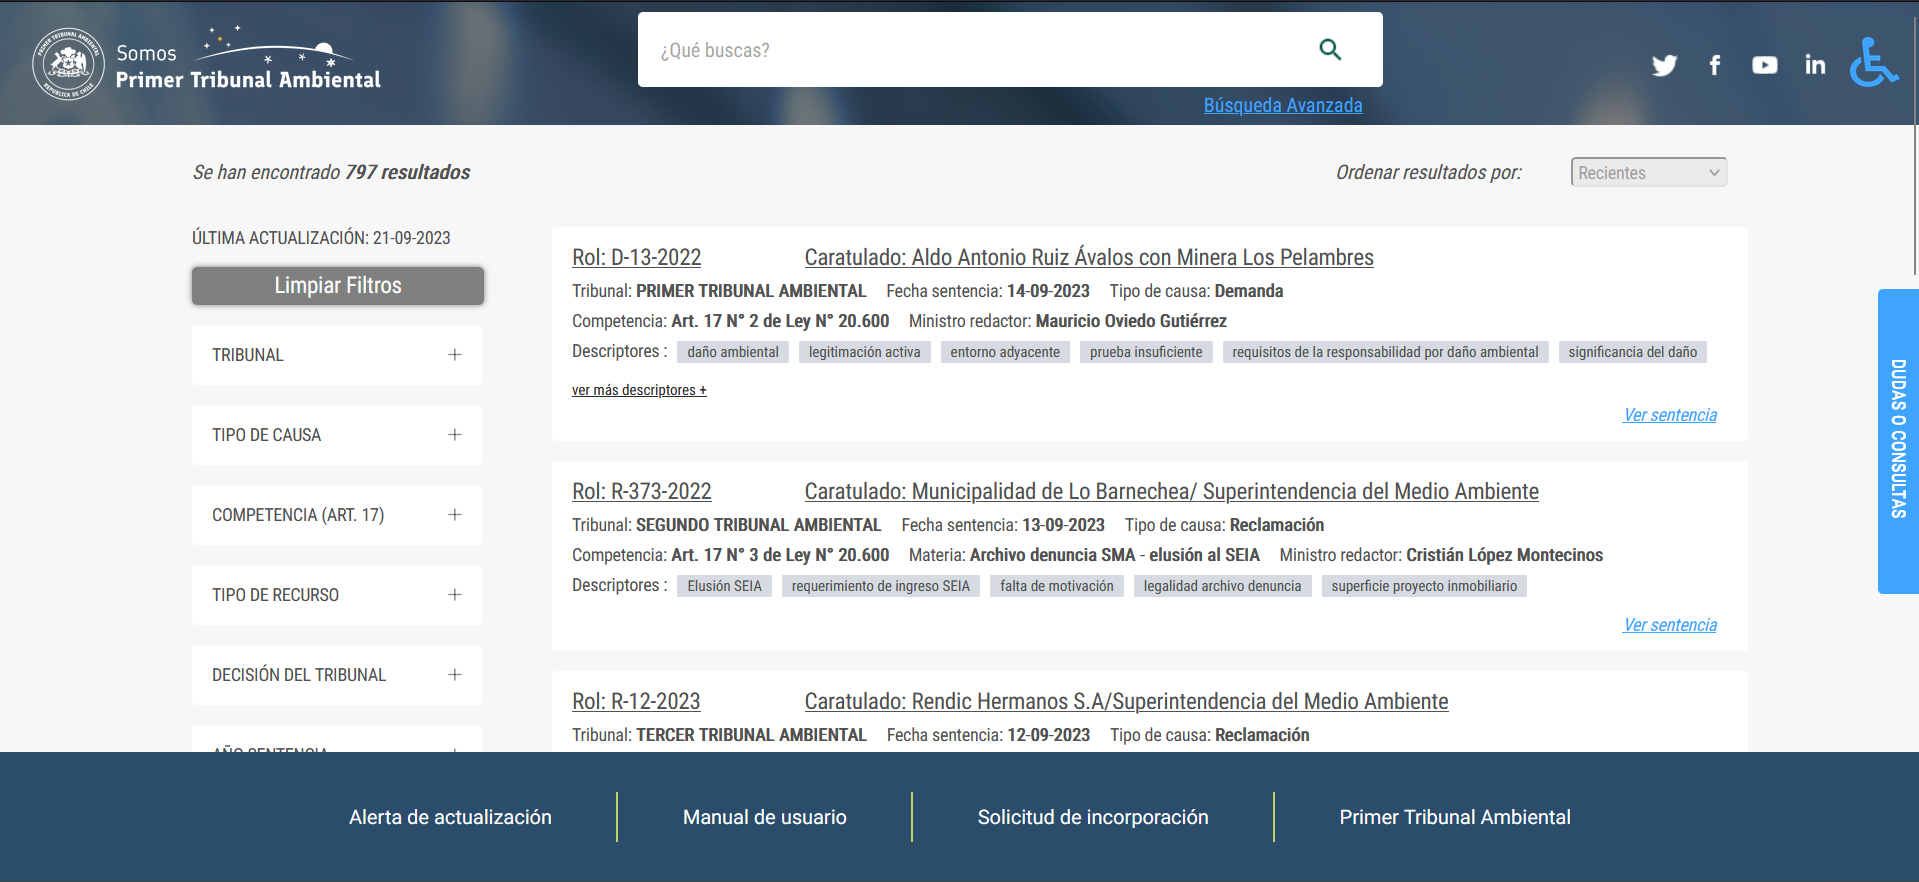
\includegraphics[width=.8\textwidth]{figures/huemul2.png}
    \caption[Screenshot del Buscador de la pagina del Primer Tribunal Ambiental]{Buscador de la pagina del Primer Tribunal Ambiental\\
    {\scriptsize (Fuente: Pagina del Primer Tribunal Ambiental)}}
    \label{fig:extract1}
\end{figure}
    
Para esta tarea, se empleó Selenium, una herramienta originalmente diseñada para generar pruebas, pero que, debido a la naturaleza 
reactiva y dinámica de los sitios web, así como a la detección de bots por parte de algunas páginas, resultó ser la elección 
más apropiada. Este bot, después de explorar todas las páginas del buscador ambiental, como se ilustra en la \autoref{fig:extract1},
logró recuperar cada uno de los enlaces individuales que conducen a las páginas específicas de cada caso, tal como se 
muestra en la \autoref{fig:extract2}.

\begin{figure}[ht!]
    \centering
    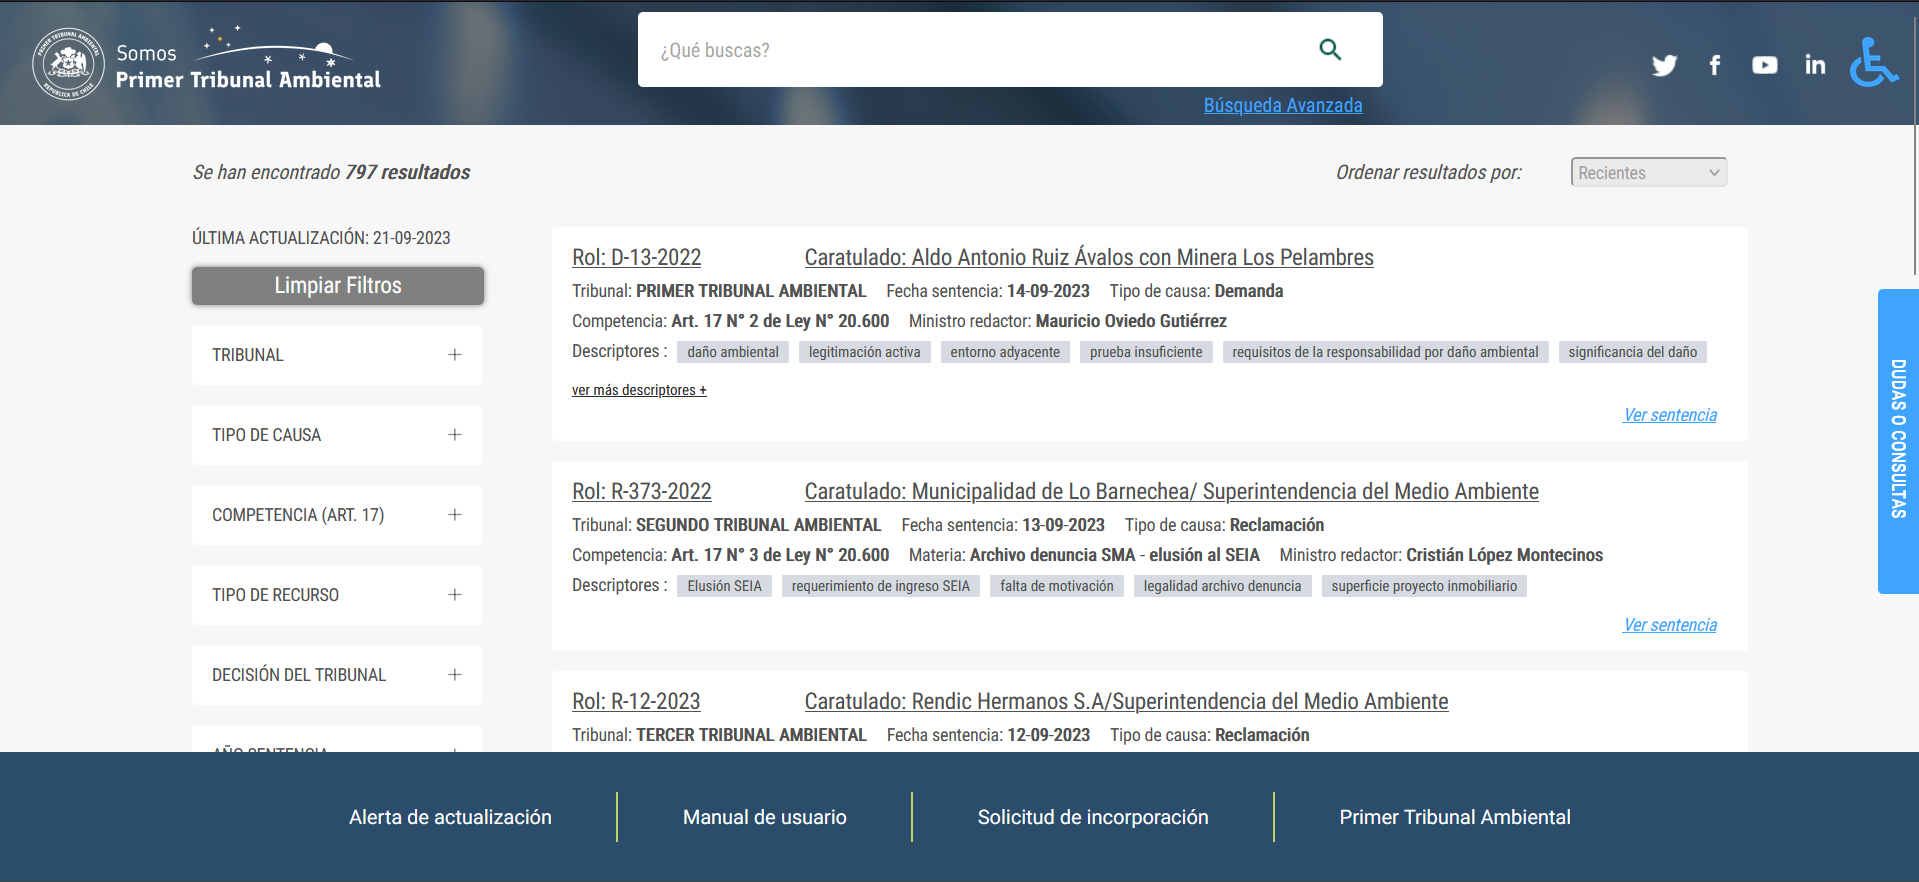
\includegraphics[width=.8\textwidth]{figures/huemul2.png}
    \caption[Screenshot de una sola reclamación en la pagina web del buscador ambiental]{Screenshot de una sola reclamación en la pagina web del buscador ambiental\\
    {\scriptsize (Fuente: Pagina del Primer Tribunal Ambiental)}}
    \label{fig:extract2}
\end{figure}
    
Posteriormente, se contemplaba la posibilidad de obtener tanto los enlaces a cada documento en formato PDF como la información 
detallada de cada uno de estos documentos mediante la creación de un nuevo bot. Sin embargo, durante el proceso de desarrollo 
de este bot, se logró acceder a la API que permitía obtener directamente todos los datos mencionados anteriormente. Esto suprimió 
la necesidad de crear otro tipo de bot utilizando Selenium, ya que bastaba con realizar una solicitud a la mencionada API.

Para completar la fase de extracción de datos (Extract), una vez que se había obtenido toda la información mediante las solicitudes 
a la API, el último paso consistió en generar nuevas solicitudes con el objetivo de descargar todos los archivos PDF de cada una 
de las entradas. Estos archivos ahora están descargados y listos para la próxima etapa del proyecto, que implica la transformación 
de los datos con el fin de obtener la información necesaria para construir la base de datos a partir de los documentos.


\subsection{Transform}

\par En la continuación del proceso de ETL (Extracción, Transformación y Carga), los PDFs que previamente han sido descargados 
requieren ser sometidos a modificaciones con el objetivo de convertir la información que inicialmente se presenta en un 
estado "sucio" en datos "limpios" que puedan ser adecuadamente utilizados en el proyecto. Este proceso se denomina 
"transformación," o "transform," en inglés.

\par Entre los datos descargados, nos encontramos con un extenso número de PDFs que presentan dificultades significativas para su 
manipulación. Esto se debe a que el Tribunal Ambiental no sigue un formato estándar en la estructura de las reclamaciones 
presentadas. En consecuencia, cada uno de los textos posee un formato propio, lo que complica en gran medida la extracción 
eficiente de las diversas secciones contenidas en dichos textos. Sin embargo, gracias al funcionamiento del proceso de semejanza 
semántica, esta diversidad de formatos no representa un problema insuperable para el proyecto.

\par No obstante, surgen dificultades adicionales cuando se trata de las reclamaciones que son presentadas a los tribunales ambientales 
en formato digital o, en su defecto, en forma de fotocopias. Esto implica que no todos los documentos están habilitados para su 
procesamiento. En consecuencia, el primer paso en el proceso de transformación involucra la discriminación de qué PDFs son 
susceptibles de ser procesados y cuáles no. Para llevar a cabo esta tarea, se ha desarrollado un script capaz de detectar 
texto dentro de un archivo PDF. Si el texto es legible, se almacena; de lo contrario, se elimina.

\par Una vez separados los PDFs legibles y adecuados para el trabajo posterior, se procede con la transformación de estos documentos 
al formato TXT (texto plano). Esta etapa se lleva a cabo considerando la conveniencia de trabajar con archivos en formato de 
texto en comparación con los archivos en formato PDF puro, dado que el próximo método de transformación, que implica el uso de
 map-reduce en Langchain, requiere que los datos estén en formato de texto.

 \par Dentro del contexto del uso de Langchain, el proceso de map-reduce implica, en primer lugar, la aplicación de una cadena de 
LLM (Modelo de Lenguaje de Gran Tamaño) a cada documento individual {docs[i]}, considerándolos de manera independiente 
(la fase de "Map"). Esto implica tratar la salida de la cadena como un nuevo documento, resumido. Posteriormente, todos los 
nuevos documentos resumidos se envían a una cadena de combinación de documentos para obtener una única salida por archivo 
(la fase de "Reduce"). En este contexto, la implementación de map-reduce en los archivos de texto (TXT) conlleva la aplicación 
de la cadena de LLM a cada documento de manera individual, generando así una nueva representación del mismo.

\par Sin embargo, es importante destacar que un archivo .txt puede contener un número de tokens demasiado elevado como para ser 
reducido de manera inmediata. En situaciones de este tipo, es necesario recurrir a un proceso de subdivisión que fragmente los 
textos en segmentos con un número de tokens inferior al límite impuesto por la API de OpenAI. Cada archivo .txt puede ser dividido, 
resumido y exportado a un nuevo archivo .txt una vez que ha sido fragmentado previamente en segmentos.

\par Los documentos procesados son combinados utilizando otra cadena de procesamiento para obtener un resultado final consolidado. 
Para concluir el proceso de transformación, los resúmenes generados después de haber pasado por el procedimiento de map-reduce 
se someten a un último paso antes de ser incorporados en la base de datos. Este paso implica la fusión de los resúmenes con la 
información obtenida a través de las solicitudes a la API del Tribunal Ambiental, presentada en formato de texto. Este proceso 
resulta en la creación de un único documento que engloba toda la información, al cual nos referiremos como "documentos finales". 
Con esto, se concluye la fase de transformación y se procede al último procedimiento, conocido como "carga" (Load), que consiste 
en cargar estos documentos finales en la base de datos.


\subsection{Load}

\par Al culminar el proceso de Extracción, Transformación y Carga (ETL), resulta fundamental llevar a cabo la fase de carga, 
también conocida como "load" en inglés, en la cual se incorporan todos los descriptores previamente descargados y transformados 
en una base de datos. Para este proyecto, en el cual se utiliza LangChain, resulta de vital importancia fragmentar los documentos 
en secciones más pequeñas.

\par Esta necesidad surge debido a que los documentos deben ser sometidos a un proceso de incrustación (embedding) antes de ser 
introducidos en la base de datos. Esto se debe principalmente a que las funciones de incrustación tienen un límite en la extensión 
de grupos de caracteres, conocidos como "tokens," que pueden ser procesados. En el contexto del modelo de incrustación 
"text-embedding-ada-002," este límite se establece en 8191 tokens [1], lo que constituye la longitud máxima de los fragmentos.

\par Por lo tanto, cuando se trabaja con documentos extensos, es imperativo dividirlos en fragmentos más pequeños antes de proceder 
con su incorporación. Según la información proporcionada en el Blog de OpenAI, los embeddings son "representaciones numéricas 
de conceptos convertidos en secuencias numéricas, lo que facilita que las computadoras comprendan las relaciones entre los 
conceptos." En términos sencillos, los embeddings son representaciones vectoriales de texto que permiten su comprensión por 
parte del Modelo de Lenguaje de Gran Tamaño (LLM). Dado que los LLM son redes neuronales, el proceso de incrustación resulta 
esencial para traducir el texto en números, que es el formato comprensible para esta red neuronal basada en Transformers.

\par Los embeddings resultantes se almacenan posteriormente en una base de datos vectorial denominada ChromaDB. Esta base de 
datos ha sido diseñada para ser compacta, escalable y eficiente, con el propósito de almacenar y recuperar vectores de manera 
efectiva. ChromaDB genera índices que permiten una recuperación rápida y eficiente de los embeddings en función de las 
consultas realizadas por los usuarios.

\section{Chatbot}

